\documentclass{beamer}
\mode<presentation>
{
	\usetheme[progressbar=foot,numbering=fraction,background=light,block=fill]{metropolis} 
	\usecolortheme{default} % or try albatross, beaver, crane, ...
	\usefonttheme{serif}  % or try serif, structurebold, ...
	\setbeamertemplate{navigation symbols}{}
	\setbeamertemplate{caption}[numbered]
	%\setbeamertemplate{frame footer}{My custom footer}
}

\usepackage{enumitem}
\usepackage{graphicx}
\usepackage{stmaryrd}
\usepackage{tikz}

\setlist[itemize]{noitemsep, topsep=-2pt, label=\textbullet}
\graphicspath{ {./figures/} }

\newcommand{\lang}{\mathcal{L}}

% Main document
\begin{document}
\title{Expressivity}
\subtitle{Dynamic Epistemic Logic}
\author[Pappas]{Thomas Pappas}
%\date{}
\maketitle

\setlength{\abovedisplayskip}{0pt}
\setlength{\belowdisplayskip}{5pt}
\setlength{\abovedisplayshortskip}{0pt}
\setlength{\belowdisplayshortskip}{0pt}

%\begin{frame}{Agenda}
  %\tableofcontents[hideallsubsections]
  %\tableofcontents
%\end{frame}

%\AtBeginSection{}

\section{Expressive power}

\begin{frame}{Expressive power}
	We'll try to answer these questions
	\begin{itemize}
		\item Which properties can be expressed with which languages and which cannot be expressed?
		\item How are languages related wrt expressivity?
	\end{itemize}
\end{frame}

\begin{frame}{Equivalence}
	\begin{block}{Definition 8.1 (Equivalence)}
		Two formulas $\phi$ and $\psi$ are \textit{equivalent} iff they are true in the same states. We denote this as $\phi \equiv \psi$
	\end{block}
\end{frame}

\begin{frame}{Expressive power}
  \begin{block}{Definition 8.2 (Expressive power)}
  	Given two logical languages $\lang_1$ and $\lang_2$ that are interpreted in the same class of models
  	\begin{itemize}
  		\item $\lang_2$ is \textit{at least as expressive} as $\lang_1$ ($\lang_1 \preceq \lang_2$)\\
  			if and only if for every formula $\phi_1 \in \lang_1$ there is a formula $\phi_2 \in \lang_2$ such that $\phi_1 \equiv \phi_2$ \pause
  		\item $\lang_1$ and $\lang_2$ are equally expressive ($\lang_1 \equiv \lang_2$)\\
  			if and only if $\lang_1 \preceq \lang_2$ and $\lang_2 \preceq \lang_1$ \pause
  		\item $\lang_2$ is more expressive than $\lang_1$ ($\lang_1 \prec \lang_2$)\\
  			if and only if $\lang_1 \preceq \lang_2$ but $\lang_1 \not\equiv \lang_2$
  	\end{itemize}
  \end{block}
\end{frame}

\begin{frame}{Expressive power: Example 1}
	Given the following languages for a countable set of propositional variables $P$
	\begin{flalign*}
		\lang_{PL} &\\
			&\phi ::= p | \neg \phi | \left(\phi \wedge \phi\right) | \left(\phi \vee \phi\right) | \left(\phi \rightarrow \phi\right) | \left(\phi \leftrightarrow \phi\right)\\
		\lang_{NAND} &\\
			&\phi ::= p | \left(\phi \barwedge \phi\right)
	\end{flalign*}
	what relation do they have wrt Expressive power?
\end{frame}

\begin{frame}{Expressive power: Example 1}
	\begin{scriptsize}
	\begin{block}{\scriptsize Theorem 8.4}
		\[\lang_{PL} \equiv \lang_{NAND}\] \pause
		\textbf{Proof.}
		\begin{itemize}
			\item $\lang_{NAND} \preceq \lang_{PL}$
				\begin{align*}
					& & t(p) &= p\\
					\phi \barwedge \psi &\equiv \neg (\phi \wedge \psi) & t(\phi \barwedge \psi) &= \neg (t(\phi) \wedge t(\psi))
				\end{align*}
			\item $\lang_{PL} \preceq \lang_{NAND}$
				\begin{align*}
				& & t(p) &= p\\
					\neg \phi &\equiv (\phi \barwedge \psi) & t(\neg \phi) &= (t(\phi) \barwedge t(\psi))\\
					\phi \wedge \psi &\equiv (\phi \barwedge \psi) \barwedge (\phi \barwedge \psi) & t(\phi \wedge \psi) &= (t(\phi) \barwedge t(\psi)) \barwedge (t(\phi) \barwedge t(\psi))\\
					\phi \vee \psi &\equiv (\phi \barwedge \phi) \barwedge (\psi \barwedge \psi) & t(\phi \vee \psi) &= (t(\phi) \barwedge t(\phi)) \barwedge (t(\psi) \barwedge t(\psi))\\
					\phi \rightarrow \psi &\equiv \phi \barwedge (\psi \barwedge \psi) & t(\phi \rightarrow \psi) &= t(\phi) \barwedge (t(\psi) \barwedge t(\psi))\\
					\phi \leftrightarrow \psi &\equiv (\phi \barwedge \psi) \barwedge (\phi \barwedge \phi) \barwedge (\psi \barwedge \psi) & t(\phi \leftrightarrow \psi) &= \dots 
						%(t(\phi) \barwedge t(\psi)) \barwedge (t(\phi) \barwedge t(\phi)) \barwedge (t(\psi) \barwedge t(\psi))
				\end{align*}
		\end{itemize}
		Show that $\phi \equiv t(\phi)$ for every formula $\phi \in \lang_{PL}$ (and $\phi \in \lang_{NAND}$ respectively) by induction on $\phi$.
	\end{block}
	\end{scriptsize}
\end{frame}

\begin{frame}{Expressive power: Example 2}
	\begin{flalign*}
		\lang_{\text{even}} &\\
			&\phi ::= p | \left(\phi \triangledown \phi\right) | \left(\phi \leftrightarrow \phi\right)\\
		\lang_{\wedge\vee} &\\
			&\phi ::= p | \left(\phi \wedge \phi\right) | \left(\phi \vee \phi\right)
	\end{flalign*}
	\begin{block}{Theorem 8.5}
		$\lang_{\text{even}} \prec \lang_{PL}$
	\end{block}
	\begin{block}{Exercise 8.6}
		$\lang_{\text{even}} \not\preceq \lang_{\wedge\vee}$ and $\lang_{\wedge\vee} \not\preceq \lang_{\text{even}}$
	\end{block}
\end{frame}


\section*{Bisimulation}

\begin{frame}{Bisimulation}
	\begin{block}{Theorem 2.15}
		For all pointed models $(M,s)$ and $(M^\prime,s^\prime)$, if $(M,s) \leftrightarroweq (M^\prime,s^\prime)$, then $(M,s) \equiv_{\lang_K} (M^\prime,s^\prime)$
	\end{block} \pause
	Does the converse hold?
\end{frame}

\begin{frame}{Bisimulation: Countably Many Atoms}
	Given a countable set of atoms P, enumarated such that $p_n$ is the $n$-th atom,
	\begin{block}{$M^1 = \langle S^1,R^1,V^1 \rangle$}
		\begin{columns}
			\begin{column}{0.5\textwidth}
				\begin{itemize}
					\item $S^1 = \{s^1\} \cup \mathbb{N}$
					\item $R^1 = \{s^1\} \times \mathbb{N}$
					\item $V^1(p_n) = \{n\}$
				\end{itemize}
			\end{column}
			\begin{column}{0.5\textwidth}
				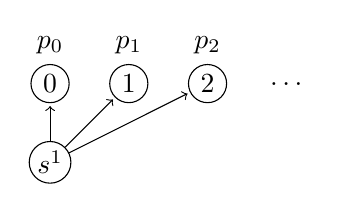
\begin{tikzpicture}[
						shorten >=1pt,
						main/.style = {draw, circle, inner sep=2pt}
					]
					\node[main,label=above:{$p_0$}] (z) {$0$};
					\node[main,label=above:{$p_1$}] (1) [right of=z] {$1$};
					\node[main,label=above:{$p_2$}] (2) [right of=1] {$2$};
					\node (d) [right of=2] {$\dots$};
					\node[main,inner sep=1pt] (s1) [below of=z] {$s^1$};
					\draw[->] (s1) to (z);
					\draw[->] (s1) to (1);
					\draw[->] (s1) to (2);
				\end{tikzpicture}
			\end{column}
		\end{columns}
	\end{block}
	\begin{block}{$M^2 = \langle S^2,R^2,V^2 \rangle$}
		\begin{columns}
			\begin{column}{0.5\textwidth}
				\begin{itemize}
					\item $S^2 = \{s^2,\omega\} \cup \mathbb{N}$
					\item $R^2 = \{s^2\} \times (\mathbb{N} \cup \{\omega\})$
					\item $V^2(p_n) = \{n\}$
				\end{itemize}
			\end{column}
			\begin{column}{0.5\textwidth}
				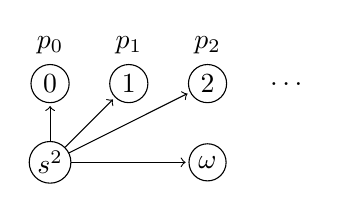
\begin{tikzpicture}[
						shorten >=1pt,
						main/.style = {draw, circle, inner sep=2pt}
					]
					\node[main,label=above:{$p_0$}] (z) {$0$};
					\node[main,label=above:{$p_1$}] (1) [right of=z] {$1$};
					\node[main,label=above:{$p_2$}] (2) [right of=1] {$2$};
					\node (d) [right of=2] {$\dots$};
					\node[main,inner sep=1pt] (s2) [below of=z] {$s^2$};
					\node[main] (om) [below of=2] {$\omega$};
					\draw[->] (s2) to (z);
					\draw[->] (s2) to (1);
					\draw[->] (s2) to (2);
					\draw[->] (s2) to (om);
				\end{tikzpicture}
			\end{column}
		\end{columns}
	\end{block}
\end{frame}

\begin{frame}{Bisimulation: Countably Many Atoms}
	$(M^1,s^1)$ and $(M^2,s^2)$ are not bisimilar (\textbf{back} is not satisfied),\\
	but $(M^1,s^1)$ and $(M^2,s^2)$ satisfy the same formulas. \pause
	%\begin{small}
	\begin{proof}
		Induction on formulas
		\begin{itemize}
			\item $s^1,s^2$ satisfy the same atoms (none)
			\item negation and conjuction are easy
		\end{itemize} \pause
		Suppose $K\phi$ a formula that could distinguish $(M^1,s^1)$ and $(M^2,s^2)$, i.e. $(M^1,s^1) \models K\phi$ and $(M^2,s^2) \not\models K\phi$ (opposite is impossible).
		\begin{itemize}
			\item $\phi$ is true in all $\mathbb{N}$ states and false in $\omega$
			\item $\phi$ is finite so let $n_{\max} = \max \{n|p_n \text{ occurs in } \phi\}$\\
				then $(M^2,n_{\max}+1) \models \phi$ iff $(M^2,\omega) \models \phi$
		\end{itemize} \pause
		Contradiction. Therefore $(M^1,s^1) \equiv_{\lang_K} (M^2,s^2)$
	\end{proof}
	%\end{small}
\end{frame}

\begin{frame}{Hedgehogs}
	\begin{figure}[h]
		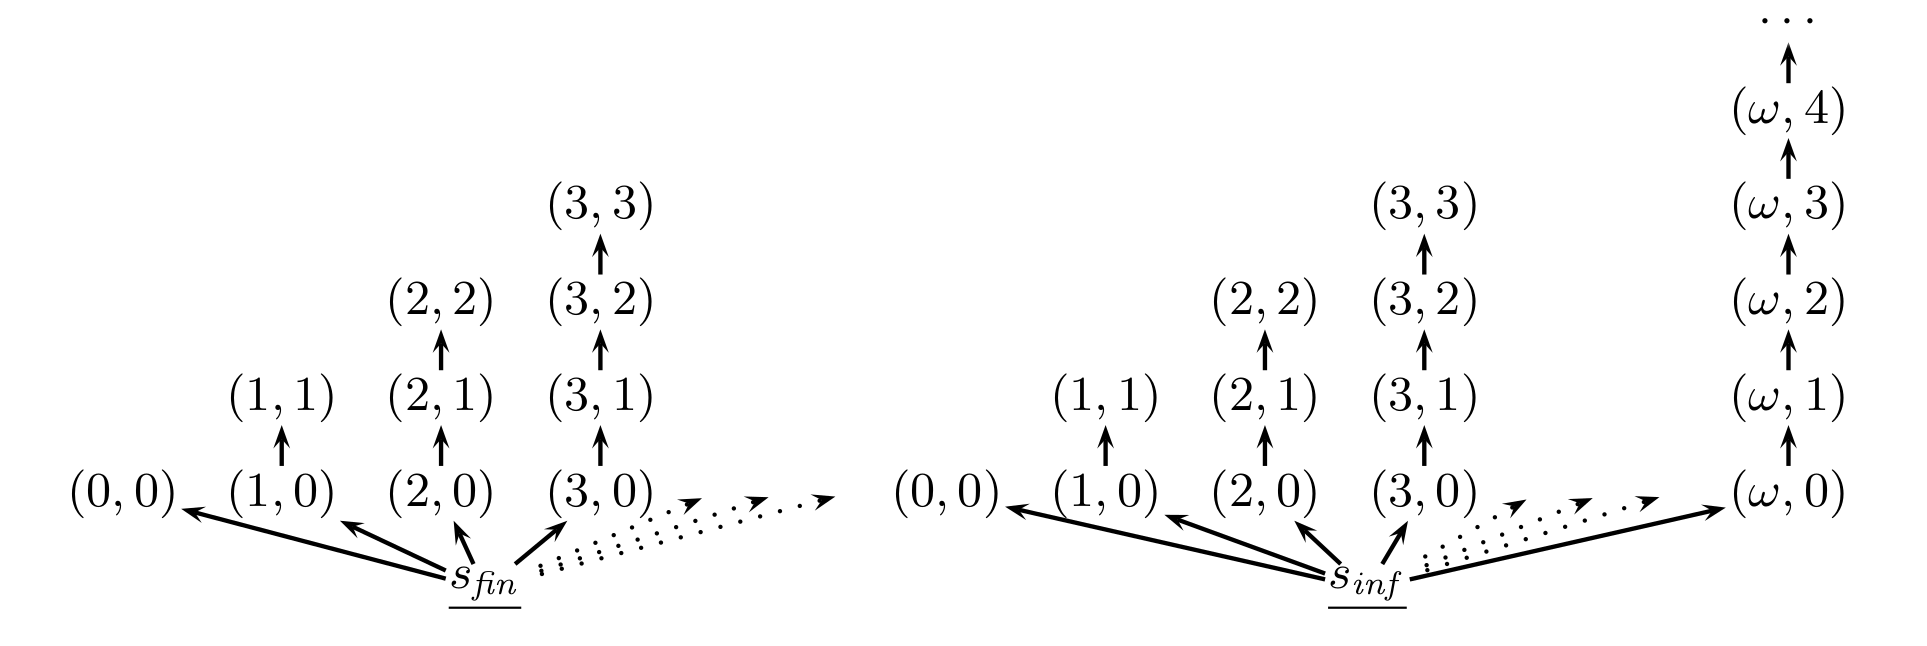
\includegraphics[width=1\textwidth]{figure_8_1_hedgehog_models}
		\caption{Left: Hedgehog with finite spines ($H_{fin}$), Right: Hedgehog with an infinite spine ($H_{inf}$).}
	\end{figure} \pause
	\begin{block}{Theorem 8.12}
		\[(H_{fin},s_{fin}) \not\leftrightarroweq (H_{inf},s_{inf})\] \pause
		\textbf{Proof.} For every $n \in \mathbb{N}$  there is a formula that distinguishes $(\omega,0)$ from $(n,0)$, i.e. the formula $(\hat{K}^n \top \wedge K^{n+1} \bot)$
	\end{block}
\end{frame}

\begin{frame}{Modal depth}
	\begin{block}{Definition 8.13 (Modal depth)}
		The modal depth of a formula is given by the function $d:\lang_K \rightarrow \mathbb{N}$ s.t.
		\begin{align*}
			d(p) &= 0\\
			d(\neg \phi) &= d(\phi)\\
			d(\phi \wedge \psi) &= \max(d(\phi),d(\psi))\\
			d(K_a\phi) &= 1 + d(\phi)
		\end{align*}
	\end{block}
\end{frame}

\begin{frame}{Hedgehogs}
	\begin{block}{Lemma 8.14}
		For the $H_{inf}$ model, for all $\phi$ s.t. $d(\phi)=n$ it is the case that\\
		$(n,0) \models \phi$ iff $(\omega,0) \models \phi$ and $(m,0) \models \phi$ for all $m>n$
	\end{block} \pause
	\begin{block}{Theorem 8.15}
		\[(H_{fin},s_{fin}) \equiv_{\lang_K} (H_{inf},s_{inf})\]
		\textbf{Proof.} Analogous to the respective proof for $(M^1,s^1),(M^2,s^2)$\\
		For $K \phi$ s.t. $(H_{fin},s_{fin}) \models K \phi$ and $(H_{inf},s_{inf}) \not\models K \phi$ we get again $(H_{inf},(\omega,0)) \not\models \phi$ and from Lemma 8.14 we get $(H_{inf},(n,0)) \not\models \phi$ where $n=d(\phi)$.
		Therefore also $(H_{fin},s_{fin} \not\models K \phi)$ which is a contradiction.
	\end{block}
\end{frame}

\begin{frame}{Finite models}
	A model is \textit{finite} iff it consists only of a finite number of states, i.e. for $M = \langle S,R,V \rangle$ then $|S| \in \mathbb{N}$.
	\begin{block}{Theorem 8.16}
		For $M=\langle S,R,V \rangle, M^\prime=\langle S^\prime,R^\prime,V^\prime \rangle$ finite models and states $s \in S, s^\prime \in S^\prime$, if $(M,s) \equiv_{\lang_K} (M^\prime,s^\prime)$ then $(M,s) \leftrightarroweq (M^\prime,s^\prime)$.
	\end{block}
\end{frame}

\begin{frame}{Finite models}
	\begin{block}{Proof.}
		Suppose $(M,s) \equiv_{\lang_K} (M^\prime,s^\prime)$, we will show the following is a bisimulation
		\[\mathfrak{R} = \{(t,t^\prime) | (M,t) \equiv_{\lang_K} (M^\prime,t^\prime)\}\]
		\begin{itemize}
			\item \textbf{atoms} Trivial
			\item \textbf{forth} For $(t,t^\prime) \in \mathfrak{R}$ and $(t,u) \in R_{\alpha}$ suppose there is\\
				no state $u^\prime$: $(t^\prime,u^\prime) \in R_{\alpha}^\prime$ and $(u,u^\prime) \in \mathfrak{R}$.\\
				Then for every such $u^\prime$ there is a formula $\phi_{u^\prime}$: $(M^\prime,u^\prime) \models \phi_{u^\prime}$ and $(M,u) \not\models \phi_{u^\prime}$.
				Now consider
				\[\phi = \bigvee_{(t^\prime,u^\prime)\in R_{\alpha}^\prime} \phi_{u^\prime}\]
			$\phi$ is finite, and we get $(M,t) \models \hat{K}_a \neg \phi$ and $(M^\prime,t^\prime) \models K_a \phi$\\
				which is a contradiction
			\item \textbf{back} Analogous to the proof for \textbf{forth}
		\end{itemize}
	\end{block}
\end{frame}

\begin{frame}{Finite degree}
	A model is said to have a \textit{finite degree} iff $\{t | (s,t) \in R_a\}$ is finite for every $s \in S$ and $\alpha \in A$, i.e. the set of accessible states is always finite.
	\begin{block}{Exercise 8.17}
		\begin{itemize}
			\item Show that there is a model of finite degree which is not a finite model.
			\item Show that Theorem 8.16 can be extended to the class of models of finite degree.
		\end{itemize}
	\end{block}
\end{frame}

\begin{frame}{Expressivity - Bisimulation}
	Notes
	\begin{itemize}
		\item Modal languages cannot distinguish non-identical models
		\item Two bisimilar models might be indistinguishable
		\item The problem seems to be related to infinity
			\begin{itemize}
				\item Formulas are finite but models may be infinite
				\item Though a theory can capture some infinitary aspects of a model, it cannot capture the whole model
			\end{itemize}
	\end{itemize}
\end{frame}

\begin{frame}
	\begin{figure}[h]
		
\includegraphics[width=1\textwidth]{i_want_to_play_a_game_meme}
	\end{figure}
\end{frame}


\section*{Games}

\begin{frame}{Games}
	A game is played with two models by two players:
	\begin{itemize}
		\item \textbf{Spoiler}: Tries to show that the models are different
		\item \textbf{Duplicator}: Tries to show that the models are the same
	\end{itemize}
	Spoiler only has a finite amount of rounds, if they fail to show that the models are different by then, the duplicator wins.
	\\[8pt]
	The two models have the same theory iff the duplicator has a winning strategy.
\end{frame}

\begin{frame}{The $\lang_K(P)$ game}
	\begin{small}
	For models $M = \langle S,R,V \rangle, M^\prime = \langle S^\prime,R^\prime,V^\prime \rangle$ and states $s \in S, s^\prime \in S^\prime$, the $n$-round $\lang_K(P)$ \textit{game} between spoiler and duplicator on $(M,s)$ and $(M^\prime,s^\prime)$ is the following \pause
	\begin{itemize}
		\item If $n=0$ then spoiler wins if $s$ and $s^\prime$ differ in any atomic property in $P$, else duplicator wins \pause
		\item If $n>0$ then spoiler can play any of the following moves
			\begin{itemize}
				\item \textbf{forth-move}: choose $a \in A, t \in S \text{ s.t. } (s,t) \in R_a$.\\
				Duplicator responds with state $t^\prime \in S^\prime$ s.t. $(s^\prime,t^\prime) \in R_a^\prime$
				\item \textbf{back-move}: choose $a \in A, t^\prime \in S^\prime \text{ s.t. } (s^\prime,t^\prime) \in R_a^\prime$.\\
				Duplicator responds with state $t \in S$ s.t. $(s,t) \in R_a$
			\end{itemize}
			Output is $(t,t^\prime)$ \pause
		\item Game continues with the new output state
	\end{itemize} \pause
	If either player cannot perform an action, that player loses\\
	If the output states differ in their atomic properties in $P$, spoiler wins\\
	If spoiler hasn't won after $n$ rounds, duplicator wins
	\end{small}
\end{frame}

\begin{frame}{Enter $\lang_K^n$}
	One should think of the number of rounds in the game as the \textit{modal depth} of the formulas the players are concerned with. \pause
	\begin{block}{Definition 8.19 ($\lang_K^n$)}
		The language $\lang_K^n$ of formulas of depth less than or equal to $n$ is defined as such
		\begin{flalign*}
			\lang_K^0 &\\
				&\phi ::= p | \neg \phi | \left(\phi \wedge \phi\right)\\
			\lang_K^{n+1} &\\
				&\phi ::= \psi | K_a \psi | \neg \phi | \left(\phi \wedge \phi\right)
		\end{flalign*}
		where $\psi \in \lang_K^n$
	\end{block}
\end{frame}

\begin{frame}{The $\lang_K(P)$ game}
	\begin{block}{Lemma 8.20}
		Given a finite set of atoms $P$, for every $n$ there are only finitely many different propositions up to logical equivalence in $\lang_K^n(P)$.\\
		\textbf{Proof.} By induction on $n$
	\end{block} \pause
	\begin{block}{Theorem 8.21}
		For all $n \in \mathbb{N}$, all models $(M,s)$ and $(M^\prime,s^\prime)$ and all finite sets of atoms $P$: duplicator has a winning strategy for the $n$-round $\lang_K(P)$-game on $(M,s)$ and $(M^\prime,s^\prime)$ iff $(M,s) \equiv_{\lang_K^n} (M^\prime,s^\prime)$.
	\end{block}
\end{frame}

\begin{frame}{The $\lang_K(P)$ game}
	\setbeamercolor{block title}{bg=}
	\setbeamercolor{block body}{bg=}
	\begin{block}{Proof.}
		Induction on $n$
		\begin{itemize}
			\item For $n=0$ it follows from the definition of the game
			\item Suppose the Theorem holds for $n$. For $n+1$
				\begin{small}
				\begin{itemize}
					\item[$(\rightarrow)$] By induction on the formula of $\phi \in \lang_K^{n+1}$
					\item If $\phi=\psi, \psi \in \lang_K^n$ it follows from (first) induction hypothesis
					\item If $\phi=K_a \psi, \psi \in \lang_K^n$, suppose $(M,s) \models K_a \psi$\\
						then for any $t^\prime: (s^\prime,t^\prime) \in R_a^\prime$ that spoiler could select,\\
						duplicator has a winning strategy, i.e. can select a $t \in R_a$: has a winning strategy in the subgame on $(M,t),(M^\prime,t^\prime)$\\[4pt]
						By induction hypothesis $(M,t) \models \psi$ iff $(M^\prime,t^\prime) \models \psi$ and since $(M,s) \models K_a \psi$ then $(M,t) \models \psi$ and $(M^\prime,t^\prime) \models \psi$\\
						$t$ was arbitrary so it holds for all $t^\prime:(s^\prime,t^\prime) \in R_a^\prime$ and therefore $(M^\prime,s^\prime) \models K_a \psi$
					\item The induction step is trivial
				\end{itemize}
				\end{small}
		\end{itemize}
	\end{block}
\end{frame}

\begin{frame}{The $\lang_K(P)$ game}
	\setbeamercolor{block title}{bg=}
	\setbeamercolor{block body}{bg=}
	\begin{block}{Proof. (cont.)}
		$(\leftarrow)$ Suppose $(M,s) \equiv_{\lang_K^{n+1}} (M^\prime,s^\prime)$, we need to describe the duplicator's winning strategy, i.e. show that for all $t: (s,t) \in R_a$ that spoiler selects, there is a $t^\prime: (s^\prime,t^\prime) \in R_a^\prime: (M,t) \equiv_{\lang_K^n} (M^\prime,t^\prime)$\\
		Then by the first induction hypothesis duplicator has a winning strategy for the remaining subgame \pause
		\\[8pt]
		Suppose there is no such $t^\prime$, so for all $t^\prime: (s^\prime,t^\prime)$ spoiler has a winning strategy, i.e. (from first induction hypothesis) there is a formula $\phi_{t^\prime}: d(\phi) \leq n$ where $(M^\prime,t^\prime) \models \phi_{t^\prime}, (M,t) \not\models \phi_{t^\prime}$
	\end{block}
\end{frame}

\begin{frame}{The $\lang_K(P)$ game}
	\setbeamercolor{block title}{bg=}
	\setbeamercolor{block body}{bg=}
	\begin{proof}[Proof. (cont.)]
		From Lemma 8.20 the set $\{\phi_{t^\prime} | (s^\prime,t^\prime) \in R_a^\prime\}$ is finite wrt equivalence.
		If $f$ a function that chooses one formula from each equivalence class $[t^\prime]$, then
		\[ \phi = \bigvee_{(s^\prime,t^\prime)\in R_{\alpha}^\prime} f([t^\prime]) \]
		is finite with $d(\phi) \leq n$ \pause
		\\[4pt]
		We have $(M^\prime,s^\prime) \models K_a \phi$ but $(M,s) \not\models K_a \phi$ while $d(K_a \phi) \leq n+1$\\
		Contradiction due to initial assumtion that $(M,s) \equiv_{\lang_K^{n+1}} (M^\prime,s^\prime)$\\
	\end{proof}
\end{frame}

\begin{frame}{The $\lang_K(P)$ game}
	\begin{block}{Theorem 8.22}
		$(M,s) \equiv (M^\prime,s^\prime)$ iff for all $n \in \mathbb{N}$ duplicator has a winning strategy for the $n$-round $\lang_K$-game on $(M,s)$ and $(M^\prime,s^\prime)$
	\end{block} \pause
	Games are finite but there are infinite games\\ \pause
	Winning strategy for duplicator coincides with bisimulation only when we consider an $\lang_K(P)$ game with $\omega$ rounds (the first ordinal limit)
\end{frame}

\end{document}
